% !TeX spellcheck = cs_CZ
\begin{example}\label{teo:exam019}
  Mějme nabitý deskový kondenzátor \(C\), zobrazený na obr. \ref{teo:fig019a}. Zvětšme jeho
  kapacitu, například tím, že zvětšíme plochu jeho elektrod, nebo připojíme paralelně druhý stejné 
  velikosti, viz obr. \ref{teo:fig019b}. Otázka zní, jak velká enerige bude uložena v 
  elektrostatickém poli obou kondeznátorů? Bude energie po rozdělení náboje mezi oba 
  kondenzátory rovna původní energií nabitého kondenzátoru? Pokud ne, vysvětlete kam se část 
  energie transformovala. 
  
   {\centering
    \captionsetup{type=figure}
    \begin{tabular}{cc}
     \subfloat[ ]{\label{teo:fig019a}
       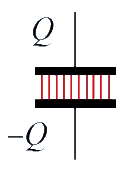
\includegraphics[width=0.15\linewidth]{teo_fig019a.png}}              &
     \hspace{3em}
     \subfloat[ ]{\label{teo:fig019b}
       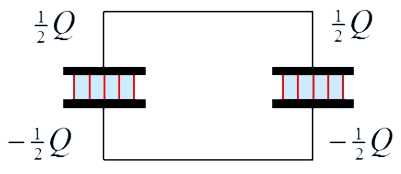
\includegraphics[width=0.5\linewidth]{teo_fig019b.png}}
    \end{tabular}
    \captionof{figure}{K příkladu \ref{teo:exam019}: a) Nabitý kondenzátor s rovnoběžnými rovinnými 
    elektrodami; b) Rozložení náboje na obou kondenzátorech velikosti}
    \label{teo:fig019}
  \par}
  
  Je-li dielektrikum kondenzátoru lineární, pak pro energii elektrického pole akumulovanou v 
  nabitém kondenzátoru platí. Podrobněji například v kapitole \ref{fyz:IIchapVsecXIX}.
  \begin{equation}
    W = \frac{1}{2}CU^2 \quad\text{nebo}\quad W = \frac{1}{2}\frac{Q^2}{C} 
    \quad\text{kde}\quad C = \frac{Q}{U}
  \end{equation}
  Předpokládejme ustálený stav po připojení druhého kondenzátoru, jak je znázorněno na obr. 
  \ref{teo:fig019b}. V obvodu nepředpokládáme přítomnost odporu, který by způsobil ztrátu energie, 
  vyzářené v podobě tepla. Kapacita je dvojnásobná a náboj zůstal stejný. Na každém kondenzátoru 
  tedy očekáváme polovinu původního náboje. Sečteme-li energii uloženou v elektrických polích obou 
  kondenzátorů dostaneme
  \begin{align*}
    W^* &= \frac{1}{2}\frac{(\frac{1}{2}Q)^2}{C} + \frac{1}{2}\frac{(\frac{1}{2}Q)^2}{C} 
         = \frac{(\frac{1}{2}Q)^2}{C} =\frac{1}{4}\frac{Q^2}{C}                               \\
        &  \xrightarrow[\scriptscriptstyle{C\rightarrow2C}]{}
           \frac{1}{2}\frac{Q^2}{(2C)} = \frac{1}{2}W 
  \end{align*}
  Kupodivu, polovina energie prostě chybí a jelikož platí zákon zachování energie\footnote{viz 
  partie Fyzika \ref{part:FYZI}, kapitola \ref{fyz:IchapII})}, nezbývá nic jiného než uznat, že 
  elektrický obvod dle \ref{teo:fig019b}, nemodeluje fyzikální problém dost věrně. Tím jsme dospěli 
  k závěru, že je nutné do obvodu dodat rezistor, tak jak je znázorněno na obrázku   
  \ref{teo:fig020}.
  
   {\centering
    \captionsetup{type=figure}
    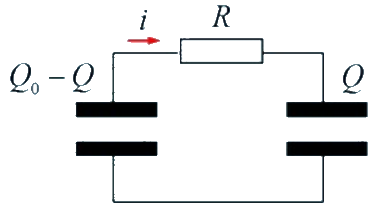
\includegraphics[width=0.4\linewidth]{teo_fig020.png}
    \captionof{figure}{Rezistor \(R\) představuje ztráty, které nebyly v obvodu na obrázku 
               \ref{teo:fig019b} předpokládány}
    \label{teo:fig020}
  \par}
  
  Abychom mohli určit teplné ztráty na rezistoru dané integrálem \(\int_{0}^{\infty} 
  Ri^2(t)\dd{t}\), nedříve sestavíme jednoduchou diferenciální rovnici prvního řádu aplikací II. 
  Kirchhoffova zákona, ze které odvodíme vzorec pro časovou závislost proudu \(i(t)\). 
  \begin{align*}
    \frac{Q_0 - Q}{C} - Ri(t) - \frac{Q_0}{C}         &= 0 \quad/\der{ }{t}             \\
    \frac{-i(t)}{C} - R\der{i(t)}{t} - \frac{i(t)}{C} &= 0                              \\
                                        \der{i(t)}{t} &= - \frac{2}{RC}i(t) \quad/\int  \\
                                                 i(t) &= I_0e^{-\frac{2}{RC}t}
  \end{align*}
  Nyní můžeme stanovit energii disipované na rezitoru \(R\)
  \begin{align*}
    W   &= \int_{0}^{\infty}Ri^2(t)\dd{t} = RI_0^2\int_{0}^{\infty}e^{-\frac{4}{RC}t}\dd{t}   \\
    \shortintertext{Do integrované funkce dosadíme novou proměnnou \(u = \frac{4}{RC}t\), \(\dd{u} 
                    = \frac{4}{RC}\dd{t}\), \(\dd{t} = \frac{RC}{4}\dd{u}\)}
        &= RI_0^2\int_{0}^{\infty}e^{-u}\frac{RC}{4}\dd{u} 
         = R^2I_0^2\frac{C}{4}\underbrace{\int_{0}^{\infty}e^{-u}\dd{u}}_1  \\
    \shortintertext{Jelikož platí \(I_0 = \frac{U}{R}=\frac{Q}{CR}\) dostaneme po dosazení}
        &= \cancel{R^2}\frac{Q^2}{C^2\cancel{R^2}}\frac{C}{4} = \frac{Q^2}{4C}
         = \frac{1}{2}W
  \end{align*}
  Nyní je vše v pořádku. Druhá polovina energie je disipována na rezistoru a navíc z výsledku 
  vyplývá, že vubec nezávisí na \(R\)!
\end{example}


